\chapter{基于内存压力的主动卸载框架}
\label{chap:基于内存压力的自动卸载框架}

在\ref{chap:基于同步内存回收的内存压力量化算法的设计与实现}中,本研究将同步内存回收延迟量化为内存压力指标。基于该量化指标,用户态的内存压力感知卸载框架能够主动将冷页面卸载到异构后端存储设备。本章将详细介绍基于proc文件系统的mpfs实现、基于内存压力的工作集动态估计算法,以及基于重用的匿名页和文件页自适应平衡回收策略的设计与实现。




\section{内存压力文件系统的实现}
\label{sec:mpfs_implementation}

基于第\ref{sec:基于同步回收延迟的内存压力量化实现}节实现的内存压力量化模型,本节构建用户态调控接口,实现系统内存资源的动态管理机制。内存压力量化提供了关键的系统状态指标,建立在此基础上的负反馈调节系统需要灵活的策略支持,以响应动态变化的资源状况。

选择在用户态实现内存压力响应策略主要基于以下理论依据与技术考量:

\begin{itemize}
    \item 策略复杂性与迭代速度:用户态环境支持实现复杂的调控策略,同时具备较短的开发、测试和部署周期,便于快速迭代优化。
    \item 差异化服务质量保障:不同应用程序对内存资源的敏感度和优先级存在差异,用户态实现便于针对特定QoS需求定制差异化的资源分配策略。
    \item 运行时可配置性:支持在系统运行过程中动态调整策略参数,无需重新编译或加载内核模块。
\end{itemize}

本节设计的 mpfs 构建了内核与用户态策略引擎之间的标准化通信接口,形成了完整的信息反馈与控制通道。

\subsection{proc文件系统架构分析}

proc文件系统作为Linux系统中内核与用户空间交互的标准机制,具备若干使其成为实现跨内核态与用户态内存压力信息交互理想媒介的特性。其动态生成机制使文件节点能够根据内核运行时状态实时动态构建;虚拟存储特性意味着不占用物理存储空间,通过内存映射实现数据存取;双向交互能力支持通过标准I/O系统调用进行内核参数查询与配置;抽象访问层则对用户态程序隐藏内核数据结构的复杂性,提供统一的访问接口。这些特性使得proc文件系统特别适合作为内核态与用户态进行内存状态交互的媒介。

\subsection{mpfs系统架构设计}

本研究设计的 mpfs 实现了三个核心功能接口: /proc/mpfs/mem\_pressure 提供实时内存压力值轮询接口并支持事件驱动的通知机制; /proc/mpfs/period 提供采样周期动态可配置接口(时间单位:秒); /proc/mpfs/mthreshold 提供修改触发阈值接口(百分比形式)。表\ref{tab:mpfs_files}详细描述了各文件接口的操作语义及功能映射关系。

\begin{table}[htbp]
    \centering
    \caption{mpfs文件系统接口规范}
    \label{tab:mpfs_files}
    \begin{tabular}{lccc}
        \toprule
        \textbf{操作类型} &  mem\_pressure  &  period  &  mthreshold  \\
        \midrule
         read  & 读取当前压力值 & 获取采样周期 & 查询当前阈值 \\
         write  & - & 更新采样周期 & 修改触发阈值 \\
         poll  & 事件通知机制 & - & - \\
        \bottomrule
    \end{tabular}
\end{table}

\begin{figure}[htbp]
  \centering
  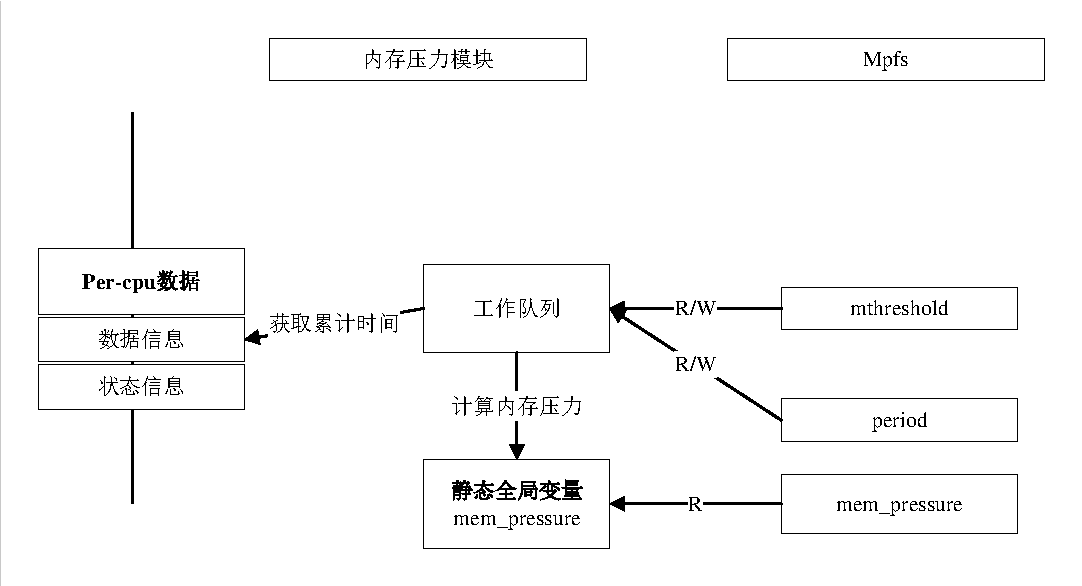
\includegraphics[width=\textwidth,keepaspectratio]{mpfs.pdf}
  \caption{mpfs与内存压力模块的交互}
  \label{fig:mpfs}
\end{figure}

图\ref{fig:mpfs}展示了mpfs与内存压力模块之间的交互架构。mem\_pressure接口在执行读取操作时通过atomic\_read()函数访问内存压力模块中的静态全局变量(atomic\_t类型),确保在多处理器环境下获取最新的内存压力值时的数据一致性。


period接口的读写操作直接影响内存压力模块中工作队列的调度参数。如第\ref{sec:consumer_implementation}节所述,系统采用Linux内核的queue\_delayed\_work()机制实现周期性的压力计算任务。当用户通过period接口修改采样周期时,系统会取消当前已排队的工作(cancel\_delayed\_work()),并使用新的时间间隔重新调度(queue\_delayed\_work(system\_wq, \&pressure\_dwork, HZ * period))。这种实现确保了采样周期的实时调整能够立即生效,同时最小化了对系统性能的影响,时间复杂度为O(1)。

mthreshold接口对阈值的读写操作同样采用原子变量(atomic\_t threshold)实现。阈值变量存储在工作队列上下文中,用于判断何时触发通知事件。内存压力计算完成后,系统通过比较当前压力值与阈值(atomic\_read(\&threshold)),当压力值超过阈值时,通过wake\_up\_interruptible()唤醒所有通过poll()系统调用等待在/proc/mpfs/mem\_pressure上的进程。选择wake\_up\_interruptible()而非wake\_up()的原因是允许等待进程响应信号,提高系统的响应性和可中断性,特别是在需要终止监控应用程序的场景下。



\subsection{内核模块实现细节}

mpfs内核模块实现基于Linux内核的proc文件系统接口机制,遵循内核模块的加载与卸载生命周期,同时提供线程安全的内存压力数据访问。以下详细阐述其核心组件设计与实现策略。

\subsubsection{文件节点与操作接口}

mpfs为用户态程序提供三个主要的proc文件接口,每个接口对应特定功能,如表\ref{tab:mpfs_files_description}所示。这些接口通过标准的 file\_operations 结构与相应的处理函数绑定,提供一致的访问语义。

\begin{table}[htbp] % 使用 table 环境,使其成为浮动体
  \centering % 将 \centering 放在 table 环境内部
  \caption{mpfs 文件节点功能说明}
  \label{tab:mpfs_files_description}
  \begin{tabularx}{\textwidth}{cX} % 使用 tabularx,并用 X 列类型
      \toprule
      \textbf{文件节点} & \textbf{功能说明} \\
      \midrule
       /proc/mpfs/mem\_pressure  & 提供内存压力值读取和事件通知功能。
      读取操作返回当前压力百分比,poll 操作支持阻塞等待压力阈值突破事件。 \\
       /proc/mpfs/period  & 提供采样周期配置接口。读取操作返回当前采样周期(秒),写入操作允许动态调整采样周期。 \\
       /proc/mpfs/mthreshold  & 提供阈值配置接口。读取操作返回当前触发阈值(百分比),写入操作允许动态设置触发阈值。 \\
      \bottomrule
  \end{tabularx}
\end{table}

读取函数通过 sprintf 格式化当前值,并使用 copy\_to\_user 安全地传递到用户空间。函数设计考虑了文件偏移量( ppos )管理,确保多次读取的正确行为。写入函数执行严格的输入验证,确保数值在有效范围内(如阈值在0-100之间),通过 kstrtofl 函数进行安全的字符串到浮点数转换,避免溢出和格式错误。

轮询函数 mempressure\_poll 通过Linux内核的等待队列机制实现事件驱动的通知模型。当用户态进程通过poll系统调用监测内存压力文件时,该函数将调用进程添加到等待队列中;当工作队列周期性计算检测到压力值超过阈值时,工作函数设置标志位并唤醒队列上的所有进程,使它们能够读取最新的压力值并执行相应策略。此设计有效避免了用户态进程频繁轮询的资源开销,提升了系统的监测效率。

\subsubsection{模块初始化与资源管理}

模块初始化函数( mpfs\_init )负责构建完整的文件系统结构。执行过程首先创建 /proc/mpfs 目录作为挂载点,然后在该目录下创建三个文件节点,并绑定相应的文件操作函数集。随后初始化单线程工作队列,避免多线程竞争带来的复杂性,并设置默认配置参数(采样周期和触发阈值)。最后调度第一次工作,启动监测循环。相应地,模块卸载函数( mpfs\_exit )负责完整的资源释放,先取消并等待所有挂起的工作完成,然后销毁工作队列,最后移除所有创建的proc文件条目。这种严格的资源管理策略确保了模块在加载和卸载过程中的稳定性和可靠性。

\subsubsection{错误处理与安全机制}

mpfs实现了全面的错误处理机制,确保系统在各种异常情况下的稳定运行。在模块初始化过程中,遵循分层式资源释放原则,任何步骤失败都会按照创建顺序的逆序释放已分配资源,有效避免资源泄漏现象。例如,在工作队列创建失败时,会自动清理已创建的proc文件节点,保持系统状态一致性。

针对用户输入安全,模块对所有通过proc文件接口传入的配置参数进行严格验证。采样周期被限制在1-600秒的范围内,阈值被约束在0-100的百分比区间,通过 kstrtofl 函数安全地将字符串转换为浮点数,防止格式错误和溢出。对于恶意输入,模块返回明确的错误码,确保即使在异常输入条件下也能维持正常运行。

为应对多核环境下的竞态挑战,关键状态更新全部采用原子操作机制。内存压力百分比和触发标志通过 atomic\_set 和 atomic\_read 函数进行操作,避免了多处理器环境下数据不一致的风险。此外,用户空间与内核空间的数据交换严格通过 copy\_to\_user 和 copy\_from\_user 函数进行,防止直接指针访问可能导致的内核内存泄露或非法访问,提供了有效的安全防护机制。

这些安全机制深度集成于各个操作函数中,形成一个多层次的防护网络,从用户输入的边界检查,到内核内部的状态保护,再到资源管理的完整性保障,mpfs通过系统化的安全设计确保在高负载、频繁访问甚至恶意使用的复杂环境下保持健壮性和稳定性。

\subsection{用户态接口应用模式}

mpfs设计的核心价值在于为用户态策略引擎提供高效且易用的系统状态访问机制。典型的使用模式包含三个主要阶段:配置阶段,应用程序通过写入配置文件设置期望的监测参数,如采样周期和触发阈值;监测阶段,应用程序通过 poll 系统调用阻塞等待压力事件,或通过周期性读取获取实时压力值;响应阶段,当接收到压力事件通知后,应用程序执行相应的资源管理策略,如内存页面卸载或应用优先级调整。

以下伪代码展示了一个简洁的用户态监测应用示例:

\begin{lstlisting}[language=C]
// 配置阶段
int fd = open("/proc/mpfs/mem_pressure", O_RDONLY);
int thfd = open("/proc/mpfs/mthreshold", O_WRONLY);
write(thfd, "5.0", 3);  // 设置5.0%为触发阈值
close(thfd);

// 监测与响应阶段
struct pollfd pfd = {fd, POLLIN, 0};
while (running) {
    // 阻塞等待内存压力事件
    poll(&pfd, 1, -1);
    if (pfd.revents & POLLIN) {
        // 读取内存压力值并执行响应策略
        float pressure;
        read(fd, &pressure, sizeof(float));
        execute_memory_management_policy(pressure);
    }
}
close(fd);
\end{lstlisting}

这种设计模式将系统状态监测与策略执行分离,使得用户态程序能够根据特定场景需求实现定制化的资源管理策略,同时不需要关心低层次的数据采集细节。通过事件驱动的监测机制,系统资源开销得到有效控制,适合在各种负载条件下长期稳定运行。

\section{基于内存压力的动态控制模型}
\label{sec:pressure_based_model}

传统的工作集估计算法主要依赖于内存分配计数器、回收事件计数器等间接指标,这些方法的有效性受限于对存储硬件特性与内核行为的专业认知要求。为解决这一问题,\ref{chap:基于同步内存回收的内存压力量化算法的设计与实现}提出了基于同步内存回收延迟的内存压力指标,该指标在不同负载模式和异构存储架构条件下表现出良好的通用性,克服了传统方法在特定场景适用性不足的缺陷。本节在此基础上,构建了一种基于内存压力的动态控制模型。该模型通过持续监测系统内存压力指标,实施主动回收策略,将内存中的冷数据页迁移至异构卸载后端中,在满足性能约束条件下,优化内存资源利用效率。

\begin{figure}[htb]
\centering
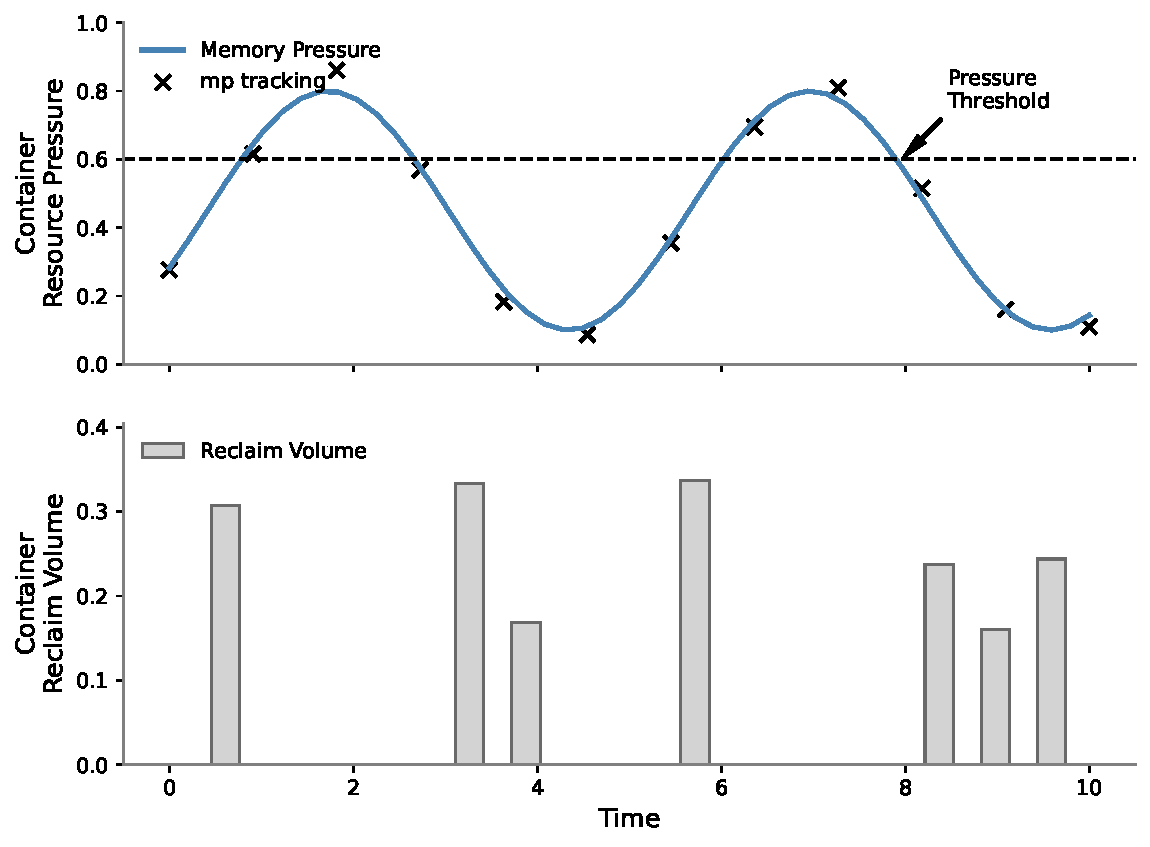
\includegraphics[width=0.95\textwidth,keepaspectratio]{压力与回收.pdf}
\caption{内存压力与页面回收控制机制}
\label{fig:pressure_work_set}
\end{figure}

图\ref{fig:pressure_work_set}展示了本模型的核心设计目标及运行机制。通过建立一个压力感知的闭环控制系统,该模型能够根据测量的内存压力值动态调整工作集大小,进而控制内存的主动卸载。当系统内存压力超过预设阈值时,模型逐步放宽内存限制以应对增长的工作集需求;反之,当内存压力低于目标值时,模型主动收紧内存限制并触发冷页面卸载,从而释放未充分利用的内存资源。这种基于压力的负反馈机制确保了系统能够在不同负载条件下维持接近最优的内存分配状态。

从经典反馈控制理论的视角看,本模型实现了闭环控制系统,以内存压力作为系统状态反馈,以内存分配大小为控制量,通过算法\ref{alg:control}动态调整控制输出。

表\ref{tab:params}列出了算法的关键参数体系,这些参数直接对应算法\ref{alg:control}中的控制变量。目标压力值(\(mem\_pressure\_target\))作为全局调控基准,默认设置为0.1\%,表示系统期望维持的内存压力。灵敏度系数(\(C_p\)和\(C_b\))控制系统对压力变化的响应程度:扩张灵敏度\(C_b = 20\)表示当实际压力达到目标值20倍时,触发最大扩容比例;收缩灵敏度\(C_p = 10\)表示当压力降至目标值1/10时,系统执行最大缩容操作。最大调整率参数(\(M_b\)和\(M_p\))限定了单次调整的幅度上限:最大扩张比例\(M_b = 1.0\)允许在单次调整中将内存限制扩大至原值的两倍,以快速响应突发性工作负载;最大收缩比例\(M_p = 0.01\)将单次缩容限制在1\%以内,确保系统稳定性并避免服务质量剧烈波动。

\begin{table}[H]
\centering
\caption{调控参数体系}
\label{tab:params}
\begin{tabular}{cccc}
\toprule
参数名称 & 符号 & 默认值 & 作用域 \\
\midrule
目标压力 & \(mem\_pressure\_target\) & 0.1\% & 全局基准值 \\
最大收缩率 & \(M_p\) & 0.01 & 缩容阶段限制 \\
最大扩张率 & \(M_b\) & 1.0 & 扩容阶段限制 \\
收缩灵敏度 & \(C_p\) & 10 & 缩容函数参数 \\
扩张灵敏度 & \(C_b\) & 20 & 扩容函数参数 \\
\bottomrule
\end{tabular}
\end{table}


算法\ref{alg:control}详细描述了基于压力量化的动态调控机制。与传统的静态内存分配策略不同,该算法通过实时内存压力指标构建了资源分配的动态反馈系统。算法以固定的时间间隔(默认为6秒)执行一次评估,通过计算当前内存压力与目标压力阈值之间的偏差来确定调整策略和幅度。

\begin{algorithm}[htb]
  \caption{Memory Pressure-Based Dynamic Control Algorithm}
  \label{alg:control}
  \Input{\(mem\_pressure\), \(mem\_pressure\_target\), \(C_b\), \(C_p\), \(M_b\), \(M_p\), \(min\_size\), \(max\_size\)}
  \Output{Memory Limit \(Limit\)}
  \While{true}{
      \(mem\_pressure \leftarrow\) Read current pressure value from mpfs interface\;
      \If{\(mem\_pressure > mem\_pressure\_target\)}{
          \(\eta \leftarrow \min\left(\left(\frac{mem\_pressure/mem\_pressure\_target}{C_b}\right)^2, 1\right) \cdot M_b\)\;
          \(Limit \leftarrow \min(max\_size, Limit \times (1 + \eta))\)\;
      }
      \Else{
          \(\eta \leftarrow \min\left(\left(\frac{mem\_pressure\_target/mem\_pressure}{C_p}\right)^2, 1\right) \cdot M_p\)\;
          \(Limit \leftarrow \max(min\_size, Limit \times (1 - \eta))\)\;
      }
      Apply new memory limit \(Limit\)\;
      Wait for next sampling period (default: 6 seconds)\;
  }
\end{algorithm}
核心调整函数采用二次函数非线性映射(第4行和第7行)将压力偏差转换为调整系数,这一设计有几个关键优势:首先,二次函数在原点附近的梯度较小,使系统对接近目标值的小偏差不过度反应,避免了因测量噪声导致的抖动;其次,当偏差增大时,二次函数的响应强度快速提升,确保对显著偏离目标状态的情况能够做出迅速响应;最后,通过\(min\)函数对调整系数进行上界约束,防止过度调整导致的系统不稳定。与简单的线性映射相比,这种非线性映射在小偏差时抑制了系统过度反应,显著偏差时又能迅速响应,从而在不同工况下表现出更好的适应性与抗干扰能力。

需要强调的是,上述算法设计具有高度可配置性,允许根据不同应用场景和性能需求进行参数调整。在高实时性要求的环境中,可以配置较高的扩张灵敏度和较低的收缩灵敏度,实现对压力增长的快速响应;而在资源受限且对性能波动容忍度较高的场景中,则可采用更积极的收缩策略以最大化资源利用率。通过这种参数化设计,算法能够适应从延迟敏感型在线服务到吞吐量导向的批处理任务等各类应用的负载特性。

此调控模型的优势在于将内存管理决策建立在直接测量的系统压力之上,而非依赖难以精确估计的工作集大小。这种方法既避免了传统启发式算法在异构系统上的适应性问题,又实现了对资源利用的精细调控。后续章节将通过延迟敏感度、资源利用率和系统吞吐量等关键指标对该模型进行全面评估,验证其在不同负载条件下的性能特性和稳定性。未来研究方向包括引入机器学习技术实现参数的自适应调整,以及将该模型扩展至更广泛的资源管理领域,如CPU、I/O带宽等多维资源的协同优化。

\section{基于重用距离的自适应页面回收策略}
\label{sec:基于重用距离的冷热页面优化}

\subsection{Linux冷热页面识别机制的局限性与改进思路}
现有的Linux冷热页面识别算法基于启发式LRU机制,该机制将文件页和匿名页区分,并使用两个独立的链表进行管理。如第\ref{sec:Linux内存回收机制}节所述,冷热页面识别算法是页面回收机制的核心组成部分。

该启发式算法最初设计面向机械硬盘存储系统。由于将匿名页卸载到机械磁盘会导致较大的换入换出开销,内核的启发式算法通常在内存不足时优先回收文件页。对于未修改的文件页,系统可以直接丢弃;对于已修改的文件页,则需写回磁盘后再释放。

然而,这种设计无法充分发挥现代异构卸载后端的性能优势。现代异构卸载后端具有显著降低的读写延迟,使得将部分匿名页卸载到这些介质上成为提高内存利用效率的可行方案。

Linux内核提供了\(swappiness\)参数来调节文件页和匿名页的回收比例,但该参数为静态超参数,需要根据经验手动设置,无法根据系统实际负载自适应调整。文件页密集型和匿名页密集型应用对\(swappiness\)参数的敏感度存在显著差异,因此系统需要能够根据实际运行环境进行动态优化。

针对这一问题,如果系统能够基于实时访问模式自适应调节\(swappiness\)参数,将有效提升整体性能。本文提出的方法核心思路为:当系统检测到文件页在短时间内被驱逐后又迅速被重新访问时(本文之后使用refault形容这种行为),表明当前工作负载可能为文件页密集型,系统将自适应调整\(swappiness\)参数,在后续页面回收过程中适当提升文件页的保留优先级,从而实现文件页和匿名页回收比例的合理分配。

本研究基于重用距离分析,构建了一种有效识别文件页短时间内refault的机制,为\(swappiness\)参数的自适应调节提供了理论依据和实现方法。

\subsection{重用距离}

设计一种通用的、高效的冷热页面识别算法具有挑战性。传统方法通常通过分析负载的特征来提出启发式的识别算法。Linux早期提出了基于重用距离(Reuse Distance)\citing{jiang2002lirs,jiang2005clockpro}的冷热页面识别算法,但由于其实现复杂度和所需额外辅助信息较多,难以在实际系统中直接应用。本研究将重用距离的概念引入页面替换策略的设计中,旨在实现文件页与匿名页回收之间的自适应平衡。重用距离能够有效刻画页面访问模式及其在页面替换中的优先级。

对于一段内存访问序列:
\[
  A \;=\;\{\,a_1,\,a_2,\,\dots,\,a_n\},
\]
其中 \(a_i\) 表示第 \(i\) 次访问的页面。令 \(P\) 为目标页面,其重用距离可以形式化地定义为:
\begin{align}
\label{eq:rd_def}
  RD(P) 
  &= 
  \min_{j>i}\Bigl\{\,j - i
    \;\Bigm|\;
    a_i = P,\;
    a_j = P,\;
    i < j
  \Bigr\}.
\end{align}

其中,\(a_i=P\) 表示第\(i\)次访问的页面为页面\(P\)。页面的重用距离与其访问频率密切相关。直观而言,若\(RD(P)\)较短,则表明页面\(P\)在近期被频繁访问,具有较高的局部性;若\(RD(P)\)较长,则表明其访问稀疏,通常可作为回收候选。

\begin{figure}[htbp]
  \centering
  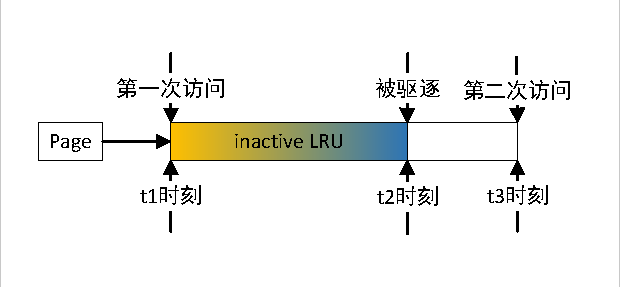
\includegraphics[width=0.8\textwidth,keepaspectratio]{重用距离.pdf}
  \caption{重用距离示意图}
  \label{fig:refault_distance}
\end{figure}


如图\ref{fig:refault_distance}所示,页面重用距离可直观理解为页面两次连续访问之间访问过的其他不同页面的数量,图中即为\(t_1\)到\(t_3\)之间被访问的不同页面数目。通过分析页面重用距离的分布,可以识别该页面的访问热度,从而及时调整页面替换策略。然而,在大规模系统中,精确计算每个页面的重用距离会引入较大的空间和计算开销,限制了其实际应用。为此,本研究提出了一种基于页面在活动链表和非活动链表间迁移行为的近似策略,通过观察页面在链表中的位置变化来间接推断其访问频度。当页面在非活动链表上被替换(即被驱逐)时,如果它在短期内再次被访问(即发生缺页异常),则说明在两次访问之间,系统至少经历了与非活动链表长度相当数量的页面访问。因此,可以通过统计缺页异常的次数和间隔来近似估计页面的访问频率。

\subsection{页面重用距离的近似计算方法}
\label{sec:重用距离的近似推导}
为了简化分析,首先假设非活动链表长度固定,并且暂不考虑活动链表向非活动链表的页面降级。此简化使得非活动链表中页面的替换和访问行为更易于形式化分析。图\ref{fig:现象1}与图\ref{fig:现象2}展示了两种核心场景。

\textbf{场景一}(图\ref{fig:现象1})呈现页框首次访问时插入非活动链表首部的置换过程。基于固定链表长度约束,原始链表中的页框发生全局尾移行为,最终触发末位页框的驱逐机制。

\textbf{场景二}(图\ref{fig:现象2})描述非活动链表页框二次访问时的状态迁移机制:当前访问页框被提升至活动链表首部,同时所有后续插入非活动链表的页框均产生位移衰减效应,其驱逐优先级按插入时序单调递增。
\begin{figure}[htbp]
  \centering
  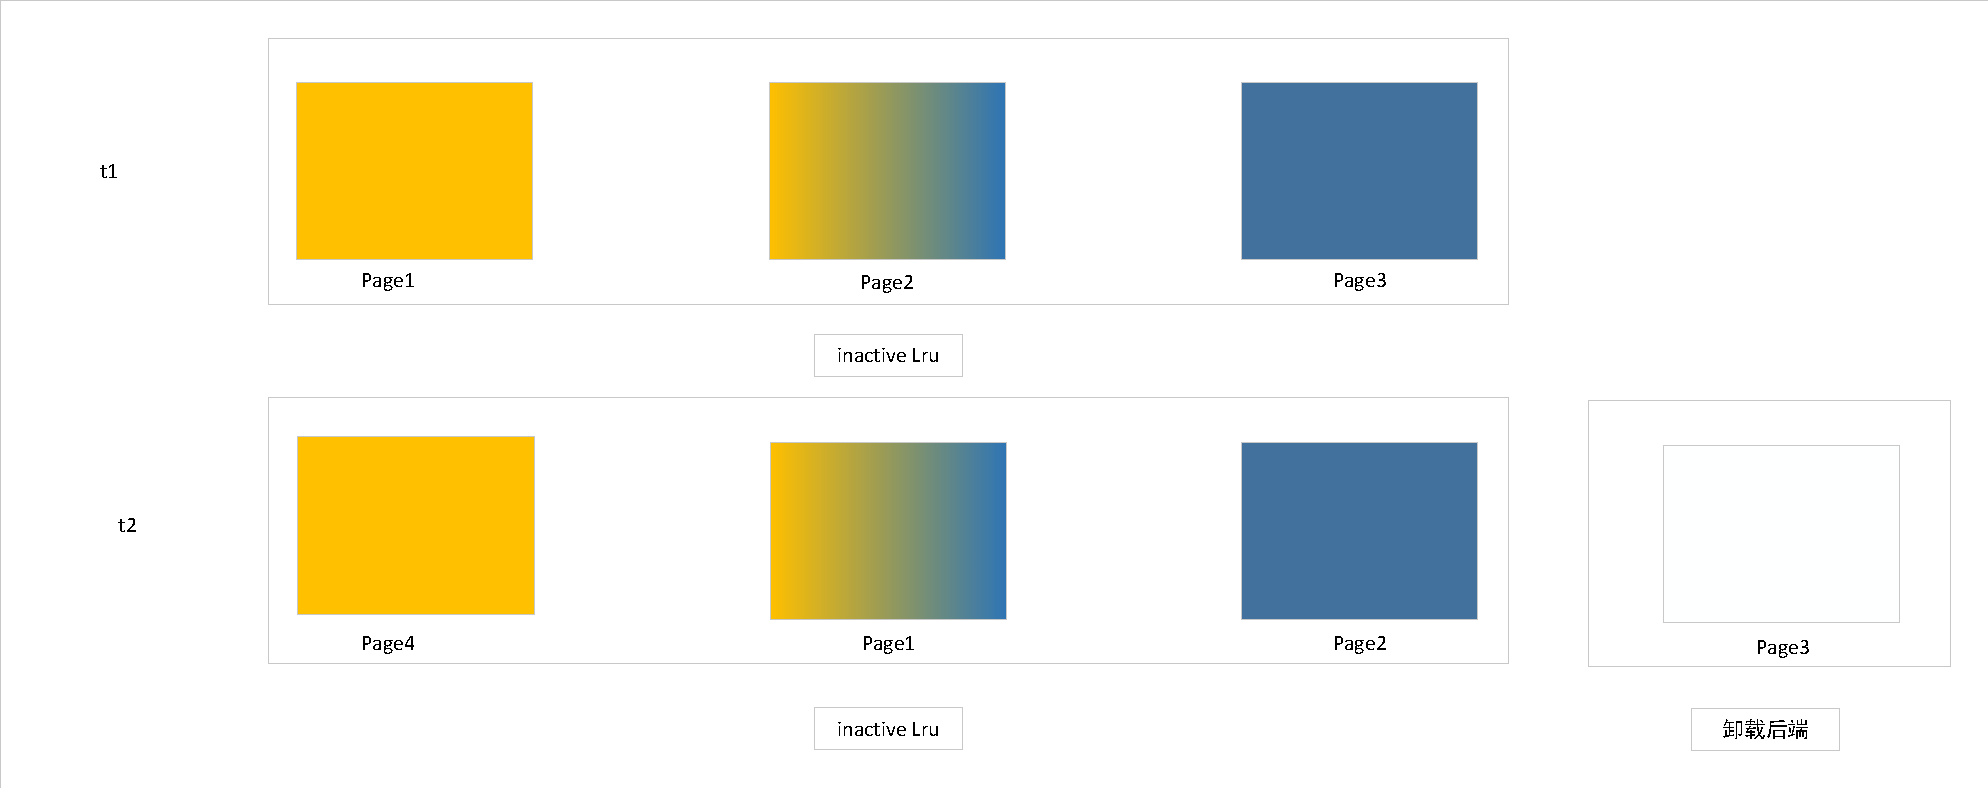
\includegraphics[width=0.8\textwidth,keepaspectratio]{现象1.pdf}
  \caption{场景一:页面首次插入非活动链表}
  \label{fig:现象1}
\end{figure}

\begin{figure}[htbp]
  \centering
  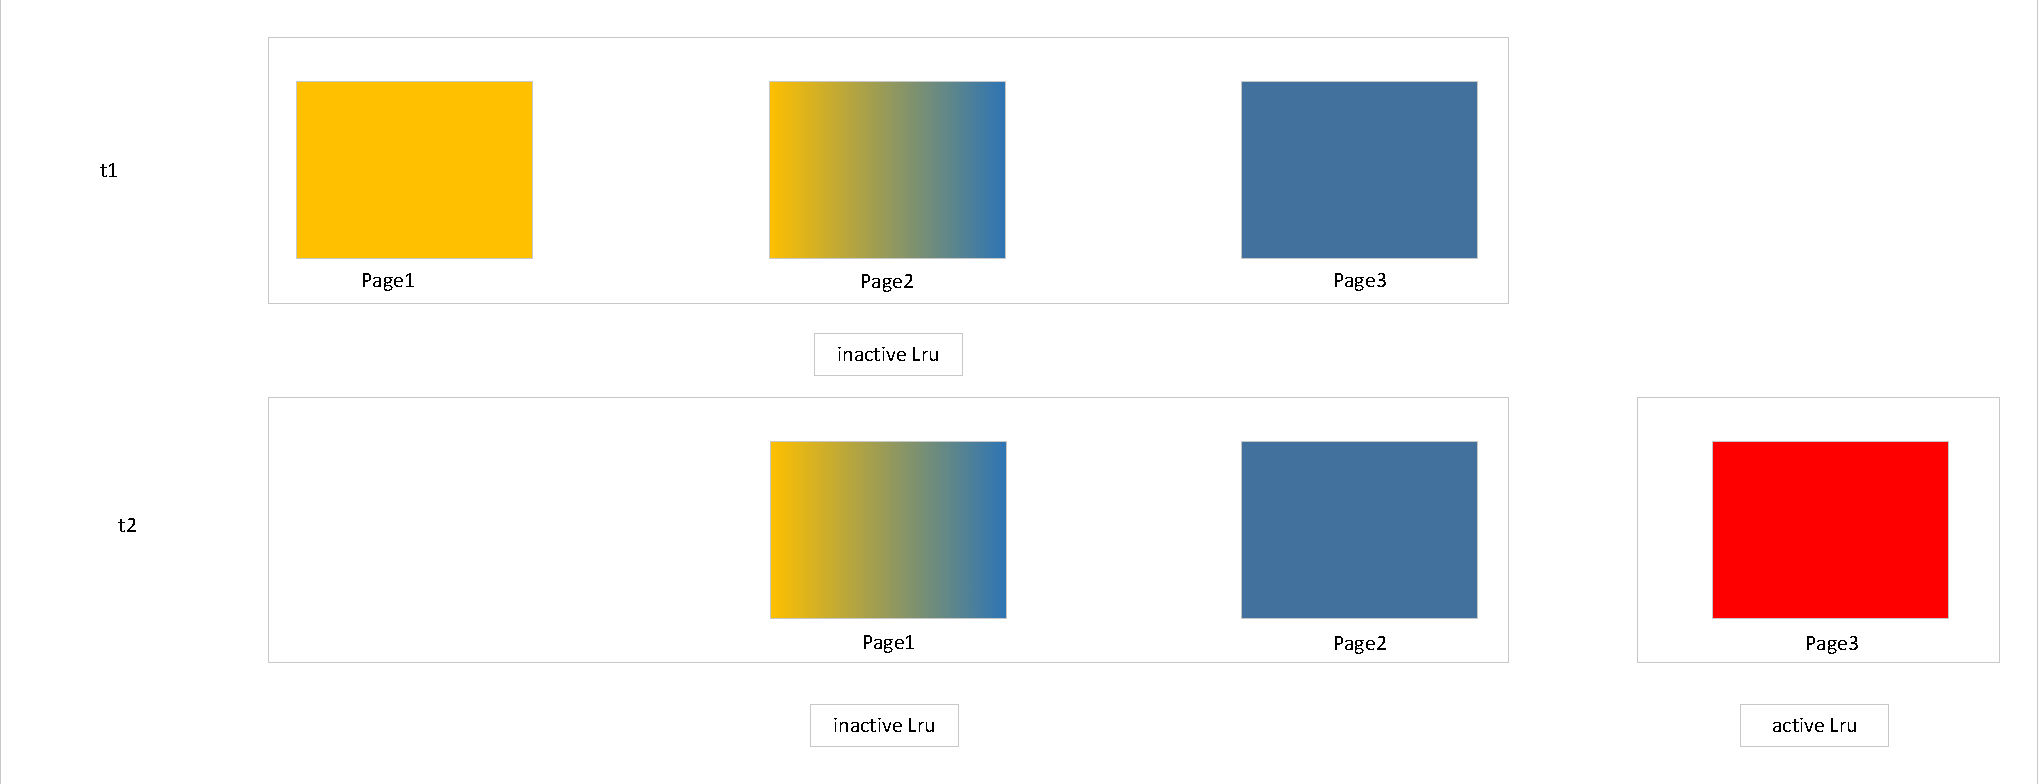
\includegraphics[width=0.8\textwidth,keepaspectratio]{现象2.pdf}
  \caption{场景二:页面在非活动链表上再次被访问并提升到活动链表}
  \label{fig:现象2}
\end{figure}

根据页面状态转移规律,在时间闭区间$[t_1, t_2]$且假设inactive\_list达到满载状态时,系统页面访问总量$V(t_1, t_2)$可解析为驱逐频次$E(t_1, t_2)$与提升频次$A(t_1, t_2)$的线性组合。该关系源于每个新增访问事件必然导致两种状态变迁之一:新页插入触发尾页驱逐,或已有页二次访问触发状态提升。可以据此建立系统页面访问总量模型:
\begin{equation}
  V(t_1, t_2) \geq E(t_1,t_2) + A(t_1,t_2)
\end{equation}
在真实系统中,还需要考虑一直停留在活动链表、从未降级的页面访问量。然而,对于访问极频繁的页面,由于其不会进入非活动链表,无需担心其再次访问情形的遗漏,因此对这部分页面的统计影响相对有限。

为了进一步验证上述理论分析的合理性,并直观展示重用距离的实际计算过程,下面通过一个具体的页面替换示例进行说明。该示例模拟了Linux双链表LRU机制下的页面访问、驱逐与提升行为,展示了如何基于系统观测到的事件序列来估计页面的重用距离。通过跟踪特定页面从首次进入内存到被驱逐再到重新访问的完整生命周期,系统可以清晰地验证前文提出的重用距离近似计算方法的有效性。

图\ref{fig:page_replacement_example}展示了Linux中的冷热页面识别机制,由活动链表和非活动链表组成,在\ref{sec:Linux内存回收机制}中介绍。图中记录了从$t_1$到$t_{10}$时间点,系统在\(p_6\)、 \(p_7\)、\(p_4\)、 \(p_8\)、 \(p_1\)、 \(p_9\)、 \(p_{10}\)、 \(p_1\)、 \(p_{11}\)、 \(p_6\)访问序列下的内存状态演变过程。该机制的核心原理是将内存页面按访问频率分为热页面和冷页面两类,分别存储于活动链表和非活动链表中。新页面首次被访问时插入非活动链表头部(如$t_1$时刻的\(p_6\));当非活动链表满时,尾部页面被驱逐(如\(t_2\)时刻的$p_3$);非活动链表中的页面被再次访问时,会被提升至活动链表头部(如$t_3$时刻的$p_4$),并将选中一个活动链表中的热页面放置到非活动链表头部(如$t_3$时刻的$p_2$)。

以页面$p_6$为例,从其在$t_1$时刻首次进入内存到$t_{10}$时刻再次被访问的过程中,系统共发生了5次页面驱逐和1次页面提升。按照重用距离的定义\ref{eq:refault_distance},页面$p_6$的重用距离为$5+1+1=7$。这里增加的1次计数来自于对活动链表中页面$p_1$的访问。虽然$p_1$位于活动链表中,其访问既不触发驱逐也不触发提升,但从系统总访问量的角度仍需计入。值得注意的是,即使活动链表中的页面偶尔被误判,但由于其访问频率高,仍能保证在内存中持续存在。
\begin{figure}[H]
  \centering
  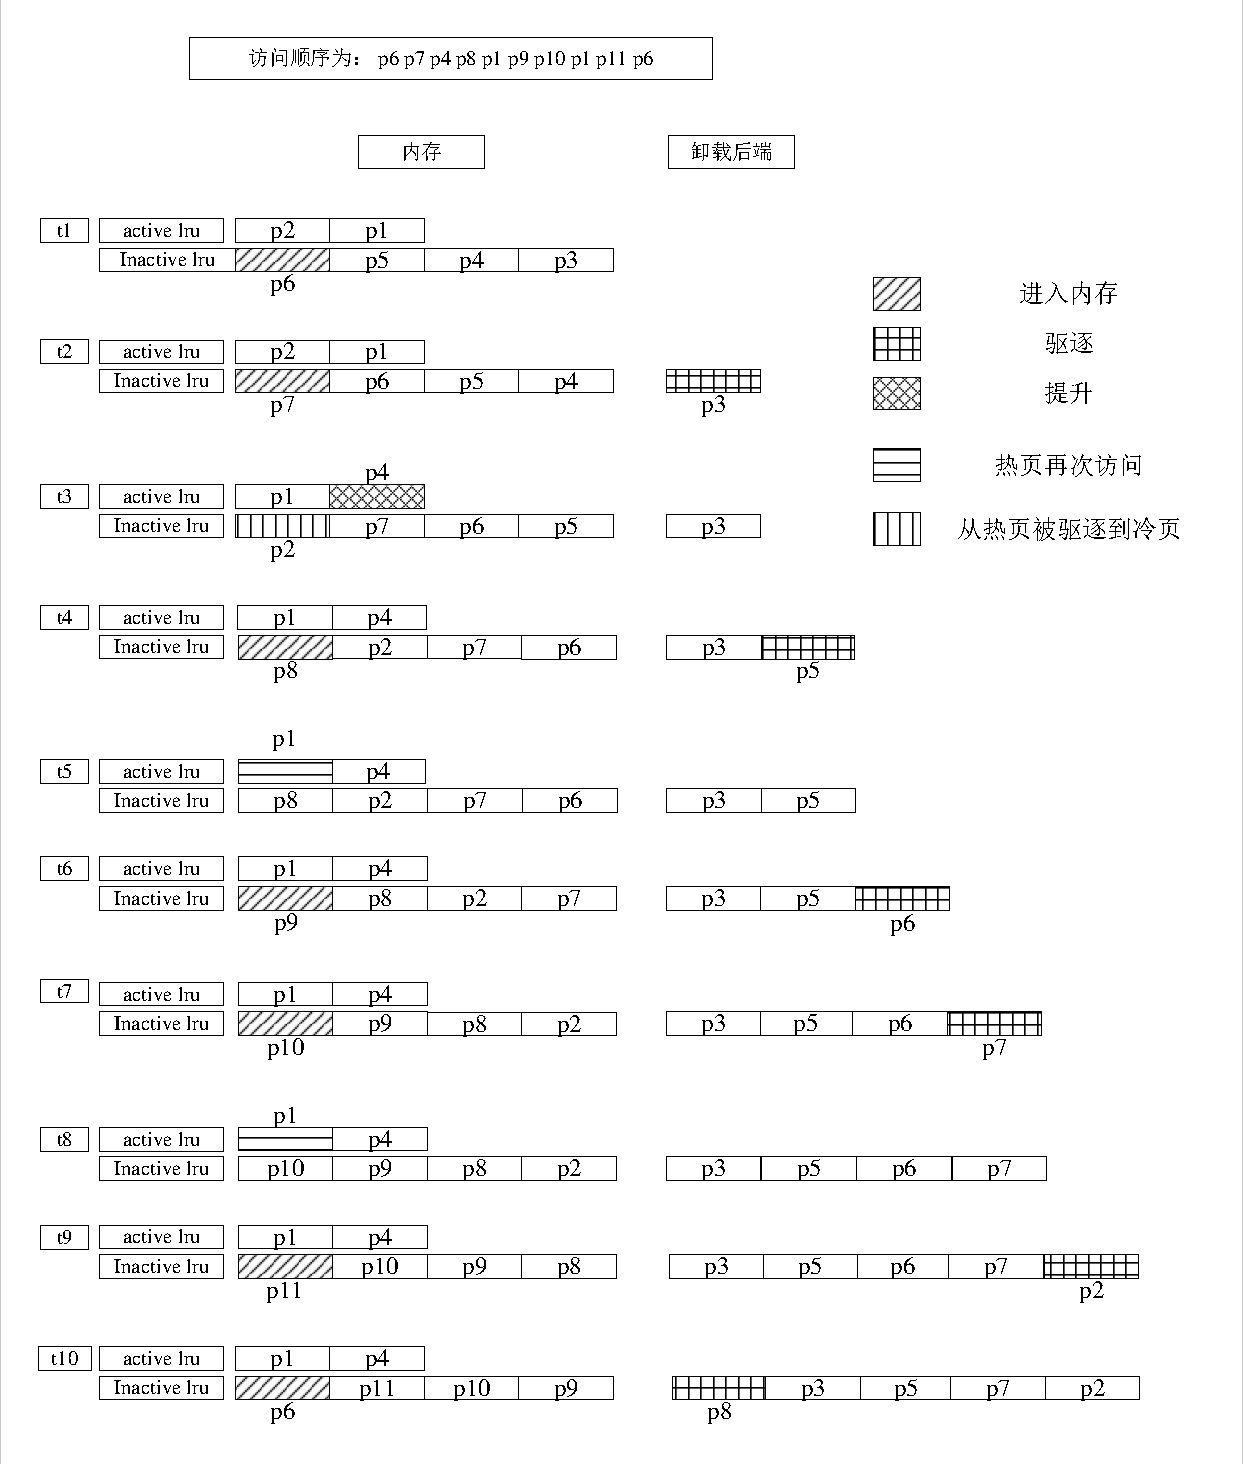
\includegraphics[width=\textwidth,keepaspectratio]{重用距离例子.pdf}
  \caption{重用距离计算示例}
  \label{fig:page_replacement_example}
\end{figure}





通过分析,可以确认使用驱逐次数和提升次数来近似估计页面重用距离的方法是合理的。观察$t_1$到$t_6$时间区间,系统共发生3次驱逐、1次提升和1次热页面访问。排除热页面访问后,驱逐次数与提升次数之和为4,恰好等于非活动链表的长度,这验证了非活动链表长度与页面访问量之间的理论关系。

在$t_7$到$t_{10}$时间区间内,系统发生了2次驱逐和1次热页面访问,但没有提升事件。对于页面$p_6$,系统可以记录其在$t_6$时刻被驱逐时的全局计数器值$count(t_6)$,以及在$t_{10}$时刻再次被访问时的计数器值$count(t_{10})$。基于这两个时刻的计数器差值,可以计算重用距离:
\begin{align}
  \label{eq:refault_distance}
  V(t_6, t_{10})
  &= 
  count(t_{10})
  \;-\;
  count(t_6).
\end{align}

该距离度量了页面$p_6$从被驱逐到再次访问期间,系统所经历的页面访问次数的下界,但不包括热页面的访问计数。

基于以上分析,可以总结:页面在非活动链表中从头部移动到尾部直至被驱逐的过程,可以近似看作经历了一系列其他页面的访问。因此,非活动链表的长度$L_{inactive}$可以作为页面在缓存中停留期间所经历的页面访问次数的估计。假设页面在$t_1$时刻被驱逐,在$t_2$时刻再次被访问,综合考虑页面在非活动链表中的移动和缺页异常期间的访问,可以得到页面$p$的总重用距离的近似形式:
\begin{align}
  \label{eq:dtotal}
  RD_p
  &= 
  L_{inactive}
  \;+\;
  \bigl(count(t_2) \;-\; count(t_1)\bigr).
\end{align}

当非活动链表长度较小时,$count(t_2) - count(t_1)$的增量会相对较大。这一现象可以从页面回收机制的角度理解:非活动链表长度较小意味着页面从进入非活动链表到被驱逐的时间间隔更短,系统内存压力更大,页面更容易被换出。在这种情况下,即使是访问频率相对较高的页面也可能在短时间内被驱逐,导致它们在被驱逐后很快又被访问,从而产生更多的缺页异常和更大的$count(t_2) - count(t_1)$值。因此,这种情况下页面需要具有更高的访问频率才能在非活动链表中停留足够长的时间而不被快速驱逐。


\subsection{基于重用距离的动态swappiness参数调节机制}

基于前述第\ref{sec:重用距离的近似推导}节中建立的重用距离理论框架及其近似计算方法,本节将深入探讨如何将这一机制应用于实际系统的内存管理优化。特别地,系统关注如何利用重用距离指标来识别refault行为模式,并以此为依据动态调整Linux内核中的\(swappiness\)参数。重用距离提供了一个量化页面访问模式的有效手段,通过公式\ref{eq:dtotal}的计算结果,系统能够准确判断页面是否在短时间内发生了refault的情况。这种refault行为往往表明系统对特定类型页面(如文件页)的回收过于激进,需要适当调整回收策略。下面,系统将详细阐述如何基于重用距离测量结果设计一种自适应的\(swappiness\)参数调节算法,以平衡文件页和匿名页的回收比例,优化系统整体性能。

可以做一下推理,如果一个页面的重用距离大于内存的,那么无论如何,该页面就是需要被驱逐。这是内存所限制了,与冷热页面识别算法无关。如果一个页面的重用距离小于内存的,那么该页面应该是要被留在内存中的。之所以被驱逐,是因为识别算法的问题,进而延伸出文件页和匿名页的回收比例问题。

所以如果页面应该保留在内存中,那么他的重用距离不应该超过内存大小,也就是不应超过活动链表和非活动链表的总长度:
\begin{align}
  \label{eq:active_condition_1}
  L_{inactive}
  \;+\;
  \bigl(count(t_2) \;-\; count(t_1)\bigr)
  &\;\;\le\;\;
  L_{inactive}
  \;+\;
  L_{active}
\end{align}

化简后可得:
\begin{align}
  \label{eq:active_condition}
  count(t_2) - {count}(t_1)
  \;\le\;
  L_{active}
\end{align}

这意味着,只有当页面的重用距离小于等于活动链表长度时,才认为其访问频率足够高,值得继续保留在内存中。

系统可以记录页面发生refault的次数,然后根据这个次数,调节\(swappiness\)参数。

算法\ref{alg:swappiness1}提出了一种基于文件页refault率动态调整Linux内核\(swappiness\)参数的机制。该算法由两个关键组件构成:refault率计算与\(swappiness\)调整逻辑。

算法的第 1-8 行定义了 CalculateFileRefaultRate 函数,该函数负责测量系统中文件页的 refault 行为。函数首先获取两个关键统计量:文件页 refault 计数(第 2 行)与文件页总数(第 3 行)。refault 计数表示被回收后又被重新访问的文件页数量,这一数据可以通过重用距离近似获得,第 \ref{sec:shadow_entry_impl} 节将详细解释。函数随后在第 4-7 行计算 refault 率,定义为每 1000 个文件页中发生 refault 的页面数量,即 \((file\_refaults \times 1000) / file\_pages\)。这种计算方式避免了浮点运算开销,同时保持了足够的精度进行决策。第 5-7 行的条件处理确保在文件页总数为零的边缘情况下算法仍能正常工作。

算法的第 9-21 行实现了 \(swappiness\) 参数的自适应调整逻辑。第 9 行调用前述函数获取当前系统的文件页 refault 率,第 10 行获取当前系统的 \(swappiness\) 值。\(swappiness\) 参数控制了系统在内存回收过程中对匿名页与文件页的回收倾向性,其取值范围为 1-150。第 11-12 行定义了 refault 率的目标区间:最小阈值 TARGET\_MIN 为 5,最大阈值 TARGET\_MAX 为 30。这两个阈值代表了系统运行的最佳状态区间,在此范围内,文件缓存的使用既不会因过度回收而导致频繁 refault,也不会因过度保留而浪费内存资源。第 13-19 行根据当前 refault 率的测量结果调整 \(swappiness\) 值。当 refault 率超过最大阈值时(第 14 行),算法减少 \(swappiness\) 值 5 个单位(第 15 行),从而降低系统对文件页的回收压力;当 refault 率低于最小阈值时(第 17 行),算法增加 \(swappiness\) 值 5 个单位(第 18 行),鼓励系统更积极地回收文件页。如果 refault 率位于两个阈值之间,则保持 \(swappiness\) 值不变,表明当前系统处于理想状态。第 20 行应用值域限制,确保调整后的 \(swappiness\) 值在 Linux 系统的有效范围内。最后,第 21 行返回调整后的值,完成一次调整周期。
\begin{algorithm}[H]
  \caption{基于文件页refault率驱动的swappiness参数调节}
  \label{alg:swappiness1}
  
  \KwIn{Current system state}
  \KwOut{Updated \(vm\_swappiness\) value}
  
  \SetKwFunction{FCalculateFileRefaultRate}{CalculateFileRefaultRate}
  \SetKwProg{Fn}{Function}{:}{}
  \Fn{\FCalculateFileRefaultRate{}}{
      \(file\_refaults \gets \text{Get file page refault count}\)\;
      \(file\_pages \gets \text{Get total file pages count}\)\;
      \eIf{\(file\_pages > 0\)}{
          \(refault\_rate \gets (file\_refaults \times 1000) / file\_pages\)\;
      }{
          \(refault\_rate \gets 0\)\;
      }
      \KwRet{\(refault\_rate\)}\;
  }
  \(fileRefaultRate \gets \FCalculateFileRefaultRate()\) \;
  \(currentSwappiness \gets \text{vm\_swappiness}\) \;  % Get the actual value
  \(TARGET\_MIN \gets 5\) \;
  \(TARGET\_MAX \gets 30\) \;

  \eIf{\(fileRefaultRate > TARGET\_MAX\)}{
      \(\text{vm\_swappiness} \gets currentSwappiness - 5\)\;
  }{
      \If{\(fileRefaultRate < TARGET\_MIN\)}{
          \(\text{vm\_swappiness} \gets currentSwappiness + 5\)\;
      }
  }
  \(\text{vm\_swappiness} \gets \max(1, \min(\text{vm\_swappiness}, 150))\) \;
  \KwRet{\(\text{vm\_swappiness}\)}
\end{algorithm}

综上所述,本研究提出的基于重用距离近似估计的页面替换策略,能够在较低开销下有效识别冷热页面,并指导文件页和匿名页的回收决策,从而提高内存利用率和系统整体性能。

\subsection{基于阴影条目的重用距离追踪内核实现}
\label{sec:shadow_entry_impl}

前文提出的基于重用距离的冷热页面识别与自适应回收算法,需要在内核中实现多个关键机制以支持其运行。本节将详细介绍全局计数维护、页面驱逐与再加载的处理流程,以及阴影条目的重用机制。

\subsubsection{全局计数维护}

为了实现基于重用距离的页面替换策略,需要在内核中维护以下关键计数信息:

\begin{enumerate}
  \item 全局的驱逐和提升次数之和(记为\(nr\_count\))。
  \item 上次缺页异常统计的次数之和(记为\(nr\_refault\_last\))。
  \item 当前时刻累积的缺页异常次数之和(记为\(nr\_refault\))。
  \item 文件页被驱逐时对应的驱逐与提升次数之和。
\end{enumerate}

其中,前三项计数直接存储在 lruvec 结构体的原子变量中,随着 lruvec 的初始化过程被设置为0。每当页面发生驱逐或提升事件时,为了保证并发访问时的计数准确性,需要对 nr\_count 执行原子递增操作。当页面再次加载时,如果满足公式\ref{eq:active_condition}的条件,则表明该页面在被驱逐后不久即被再次访问,此时系统会将其视为一次缺页异常,并相应地增加 nr\_refault 计数。通过计算 nr\_refault 和 nr\_refault\_last 的差值,可以动态评估文件页的这段时间发生refault的次数,进而通过算法\ref{alg:swappiness1}调整文件页和匿名页的回收比例。

\subsubsection{基于阴影条目的重用距离追踪机制}
\label{sec:shadow_entry}
为了实现基于重用距离的页面替换策略,核心挑战在于:如何在页面被驱逐后,仍能记录其驱逐时刻的全局计数值\(count(t_1)\),以便在页面再次载入时计算重用距离。直接为每个被驱逐的页面单独分配存储空间记录这些信息显然不现实,这将带来大量额外的内存开销和复杂的生命周期管理问题。

本研究的关键创新在于发现了一种零额外内存开销的解决方案:复用Linux内核 page cache 中前缀树的数据结构特性。这一方案基于以下两个关键观察:

\begin{enumerate}
  \item 在Linux内核中,当页面被驱逐后,其在前缀树中的槽位将变为空闲状态。
  \item  struct page 在内存中是按照16字节对齐的,这意味着 struct page 指针的低4位始终为0,其中低2位可以安全地用作标志位而不影响指针的寻址功能。
\end{enumerate}

Linux内核已经使用指针的低2位作为内部状态标志(00表示普通页面,01表示页面锁定等)。经过详细分析内核代码,发现位模式10尚未被使用,因此选择该模式作为阴影条目的标识,既避免了与现有内核机制的冲突,又保留了一定的扩展空间。

基于上述观察,本文复用了阴影条目(shadow entry)机制:当页面被驱逐时,不是简单地将其前缀树槽位清空,而是将当前的全局计数值(\(count(t_1)\))左移两位后存入该槽位,并将低两位设置为10标志,表示这是一个阴影条目而非有效页面指针。这样,阴影条目既保存了页面驱逐时的关键信息,又不需要额外的内存分配。

\begin{figure}[htbp]
  \centering
  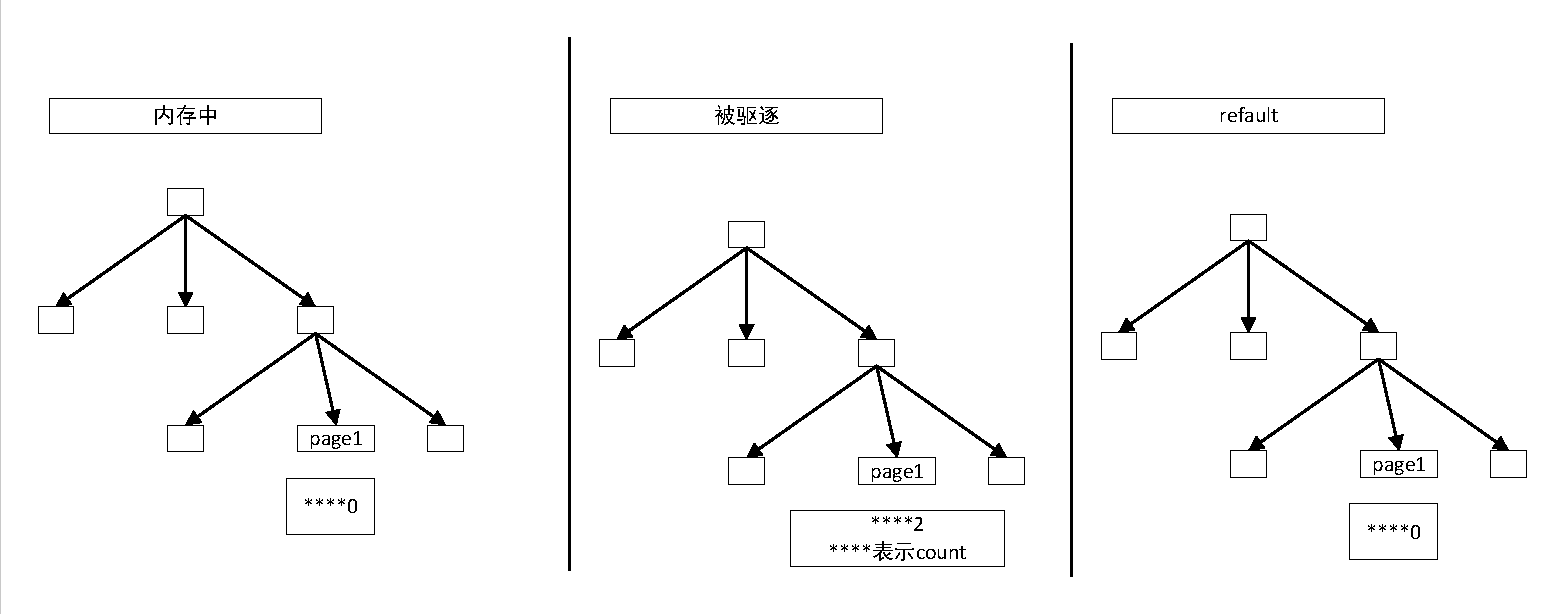
\includegraphics[width=\textwidth,keepaspectratio]{复用.pdf}
  \caption{阴影条目机制:利用前缀树指针槽位复用存储驱逐时的全局计数值}
  \label{fig:复用}
\end{figure}

如图\ref{fig:复用}所示,可以看到在页面生命周期的不同阶段,前缀树槽位存储的指针具有不同的状态:当页面在内存中时,前缀树槽位存储指向 struct page 的正常指针(标志位00);当页面被驱逐后,槽位转变为阴影条目,存储驱逐时的全局计数值(标志位10);当页面再次加载的时候,前缀树槽位再次存储指向 struct page 的正常指针(标志位00)。此时配合全局计数器\(nr\_count\),可以计算出页面在驱逐后的访问的页面的数量。详细实现步骤如下:

在页面驱逐阶段(\_\_remove\_mapping函数中):
\begin{enumerate}
  \item 原子读取当前全局计数器\(nr\_count\)的值
  \item 将计数器值左移两位,为标志位预留空间
  \item 通过按位或操作设置低两位为 10 ,生成阴影条目
  \item 将阴影条目存入前缀树对应槽位,替换原页面指针
  \item 原子递增全局计数器\(nr\_count\),记录驱逐事件
\end{enumerate}

在页面再次加载阶段(pagecache\_get\_page函数中):
\begin{enumerate}
  \item 检查前缀树槽位的低两位,判断是否为阴影条目( 10 )
  \item 若为阴影条目,提取存储的计数值(右移两位)作为\(count(t_1)\)
  \item 获取当前全局计数器值作为\(count(t_2)\)
  \item 根据公式\ref{eq:active_condition}判断页面是否应提升至活动链表
  \item 更新相关统计计数并清除阴影条目,替换为新加载页面的指针
\end{enumerate}

此外,为了保证高并发环境下的一致性,本文为阴影条目的读写操作添加了适当的内存屏障指令。在多处理器系统中,使用smp\_wmb()确保计数值写入前缀树槽位的操作对其他CPU核心可见,而使用smp\_rmb()确保读取操作能获取最新的计数值。这些同步措施与Linux内核已有的radix-tree锁机制配合,保证了阴影条目在并发访问下的数据一致性。

这种设计巧妙地利用了指针对齐的特性,在不增加内存开销的情况下,实现了对页面重用距离的有效追踪。通过阴影条目存储的历史信息,系统能够识别哪些页面在驱逐后迅速被再次访问(热页面),从而优化页面替换策略,提高内存利用效率。


\subsubsection{Shrinker回收机制}

在上一节\ref{sec:shadow_entry}中,本文详细介绍了如何通过重用前缀树指针的低位标志位来存储页面驱逐时的全局计数器值,从而实现页面访问历史的有效追踪。然而,这种优化技术虽然减少了元数据存储开销,却会导致前缀树中的阴影条目不断累积。阴影条目是指那些对应的实际页面已被驱逐,但其元数据仍保留在前缀树中的节点。若不及时清理这些阴影条目,将导致前缀树结构过度膨胀,占用过多的系统内存资源。

为了解决阴影条目累积导致的内存浪费问题,本研究利用Linux内核提供的Shrinker机制实现对阴影条目的自动回收。Shrinker是Linux内核内存回收子系统中的统一回调接口,用于管理内核缓存对象(如inode、dentry等)的回收。此机制通过struct shrink\_control(表\ref{tab:shrink_control_struct})与struct shrinker(表\ref{tab:shrinker_struct})两个核心数据结构向回收框架注册接口。内核在低内存或内存压力较大时主动调用已注册的shrinker接口,以回收可释放的内核缓存对象。

\begin{table}[htbp]
  \centering
  \caption{struct shrink\_control 结构体主要字段说明}
  \label{tab:shrink_control_struct}
  \begin{tabular}{ccc}
    \toprule
    \textbf{成员} & \textbf{类型} & \textbf{说明} \\
    \midrule
    gfp\_mask & gfp\_t & 本次内存分配的掩码,指示约束条件 \\
    nid & int & 所在的 NUMA 节点 \\
    nr\_to\_scan & unsigned long & 期望本轮扫描并回收的对象数 \\
    nr\_scanned & unsigned long & 实际扫描对象数量 \\
    memcg & struct mem\_cgroup * & 针对特定 memcg 的回收(若有) \\
    \bottomrule
  \end{tabular}
\end{table}

\begin{table}[htbp]
  \centering
  \caption{struct shrinker 结构体主要字段说明}
  \label{tab:shrinker_struct}
  \begin{tabular}{ccc}
    \toprule
    \textbf{成员} & \textbf{类型} & \textbf{说明} \\
    \midrule
    count\_objects & 函数指针 & 返回可回收对象数,若无可回收则返回 SHRINK\_EMPTY \\
    scan\_objects & 函数指针 & 实际扫描并回收对象,返回已释放数量 \\
    batch & long & 每次回收的批次大小,默认为 0(使用默认值) \\
    seeks & int & 反映对象重建开销,影响回收优先级 \\
    flags & unsigned & Shrinker 能力标志(NUMA 感知等) \\
    list & struct list\_head & 内核内部使用,用于将 shrinker 链接到全局列表 \\
    id & int & 在 memcg 上下文中的 shrinker 标识 \\
    nr\_deferred & atomic\_long\_t * & 延迟对象数计数 \\
    \bottomrule
  \end{tabular}
\end{table}

本研究实现的回收机制通过精细分类前缀树节点,提高了回收的效率和精确性。如图\ref{fig:shrink}所示,将前缀树节点分为三类:


\begin{enumerate}
  \item 常规页面节点(图中白色方块):仅包含对应有效物理页面的条目,这类节点不参与回收。
  \item 部分Shadow节点(图中斜线方块):同时包含阴影条目和常规页面条目的混合节点,由于其中仍含有有效页面信息,暂不进行回收。
  \item 完全Shadow节点(图中灰色方块):节点内全部条目均为阴影条目,没有对应任何当前有效的物理页面,是回收的主要目标。
\end{enumerate}
scan\_objects函数实现采用双重优化策略:首先,仅针对完全 Shadow 节点进行回收,避免影响正常页面访问;其次,利用Linux内核的LRU链表机制组织这些完全 Shadow 节点,形成高效的回收队列。如图\ref{fig:shrink}所示,LRU链表按照节点最后访问时间排序,使得系统能够在\( O(1) \) 时间复杂度内识别并回收最长时间未被访问的完全Shadow节点。
\begin{figure}[htbp]
  \centering
  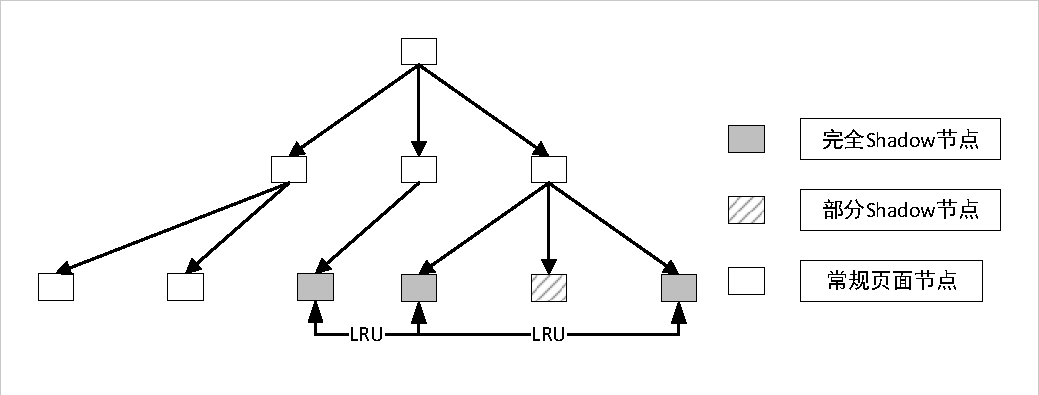
\includegraphics[width=\textwidth,keepaspectratio]{Shrinker设计.pdf}
  \caption{Shrinker机制工作原理示意图}
  \label{fig:shrink}
\end{figure}
当前缀树节点的所有条目转变为阴影条目时,该节点会被自动添加到专用的LRU链表尾部。随后,当节点在LRU链表中移动到头部位置时,如果仍保持完全Shadow状态,则成为优先回收的候选对象。这种设计不仅避免了对整个前缀树的遍历开销(避免\(O(n)\)的扫描复杂度),还能确保回收操作优先针对长时间未访问的节点,保留近期可能重新访问的页面历史信息。

count\_objects函数负责估算可回收的阴影条目数量。它根据系统当前的内存压力水平采用自适应算法动态计算合理的阴影节点数量上限。具体而言,在低内存压力条件下,允许保留更多阴影节点以优化缓存命中率;而在高内存压力条件下,则提高回收阈值以释放更多内存资源。这种动态平衡策略在内存效率与访问性能之间取得了较好的折中。

\section{本章小结}
\label{sec:本章小结}

本章详细介绍了基于内存压力的自适应主动冷页面卸载框架的设计与实现。首先,介绍了利用proc文件系统实现的mpfs模块,提供了用户态与内核态之间的标准交互接口。mpfs模块允许用户态程序实时获取内存压力信息,并动态调整采样周期和压力阈值,为用户态的调控策略提供了基础。随后,提出了基于内存压力的动态调控模型,利用负反馈机制,根据实时内存压力动态调整内存使用范围,实现了主动的冷页面卸载。该模型通过参数化设计,可以灵活适应不同的应用场景和性能需求。最后,详细介绍了基于重用距离的自适应页面回收策略。通过近似计算页面的重用距离,实现了文件页和匿名页的自适应平衡回收。为了支持该策略,本研究在内核中实现了全局计数维护、阴影条目管理和Shrinker回收机制。通过重用前缀树指针的低位标志位,避免了在 struct page 结构中引入额外字段,最大程度地减少了内存开销。

本章提出的框架和算法,为实现高效、自适应的内存管理提供了可行的方案。通过将内存压力作为核心调控指标,结合重用距离进行页面回收决策,能够在保证系统性能的同时,显著提高内存资源的利用率。未来的研究方向包括引入机器学习技术实现参数的自适应调整,以及将该模型扩展至更广泛的资源管理领域。
